\documentclass{article}
\usepackage[margin=0.5in]{geometry}
\usepackage{tikz}
\usepackage{graphicx}
\usepackage{listings}

\title{SPIDR Analysis Documentation}
\author{Darvesh Gorhe, Ahmed Abdou, Erica Wolin}

\begin{document}
    \maketitle
    \tableofcontents

    \section{Introduction}
    This document will outline the analysis pipeline for the SPIDR project. The pipeline is divided into three main sections: preprocessing, post-pipeline, and downstream analysis. The preprocessing section will outline the steps taken to go from fastq files to bed files. The post-pipeline section will outline the steps taken to prepare the data from bed files to bedgraph files. The downstream analysis will outline the steps taken to analyze the data from bedgraph files to the final results.
    \vspace{5mm}

    \noindent The preprocessing and the postprocessing pipeline use Snakemake to orchestrate several steps in an efficient way using \texttt{sbatch} jobs. These \texttt{sbatch} jobs are ways to run individual sections of the pipeline on high-performance computing clusters.

    \section{Preprocessing Pipeline}
    \subsection{Overview}

    \begin{figure}[ht!]
        \centering
        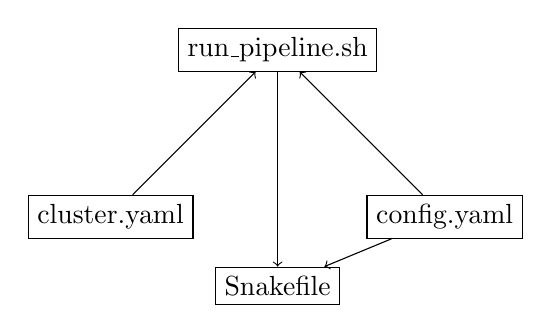
\begin{tikzpicture}
            % Nodes
            \node[draw] (run_pipeline) {run\_pipeline.sh};
            \node[draw, below left of=run_pipeline, node distance=3cm] (cluster_yaml) {cluster.yaml};
            \node[draw, below right of=run_pipeline, node distance=3cm] (config_yaml) {config.yaml};
            \node[draw, below of=run_pipeline, node distance=3cm] (Snakefile) {Snakefile};
            
            % Arrows
            \draw[->] (cluster_yaml) -- (run_pipeline);
            \draw[->] (config_yaml) -- (run_pipeline);
            \draw[->] (run_pipeline) -- (Snakefile);
            \draw[->] (config_yaml) -- (Snakefile);
        \end{tikzpicture}
        \caption[short]{Overview of preprocessing configuration.}
    \end{figure}

    \noindent Above we see an overview of the primary files involved in configuration of the preprocessing pipeline. \texttt{run\_pipeline.sh} is the shell file that actually gets called to run the pipeline. \texttt{cluster.yaml} is the file that configures the \texttt{sbatch} jobs. It sets things like the account ID so jobs actually get queued, the memory per job, the number of cpus per job, the maximum time a job should run, etc. \texttt{config.yaml} is the file that configures the pipeline itself. This has parameters like the filepaths for indicies for the bowtie2 and STAR aligners. \texttt{Snakefile} is the file that actually runs the pipeline and contains all the rules. The rules are the individual steps that are run in the pipeline. 
    \vspace{5mm}
    
    \noindent Rules are chained together automatically based on the name of input and output file specified within each rule. Snakemake will create a directed acyclic graph (DAG) upon launching the pipeline. A DAG is a data structure which tells Snakemake the dependencies between rules so Snakemake can determine how to optimally schedule rules on a system. Snakemake will then run the rules in the correct order and in parallel when possible. Below is an example of a DAG for the preprocessing pipeline with \texttt{num\_chunks}$=2$. As the number of chunks becomes larger, the middle of the graph becomes correspondingly wider.

    \begin{figure}[ht!]
        \centering
        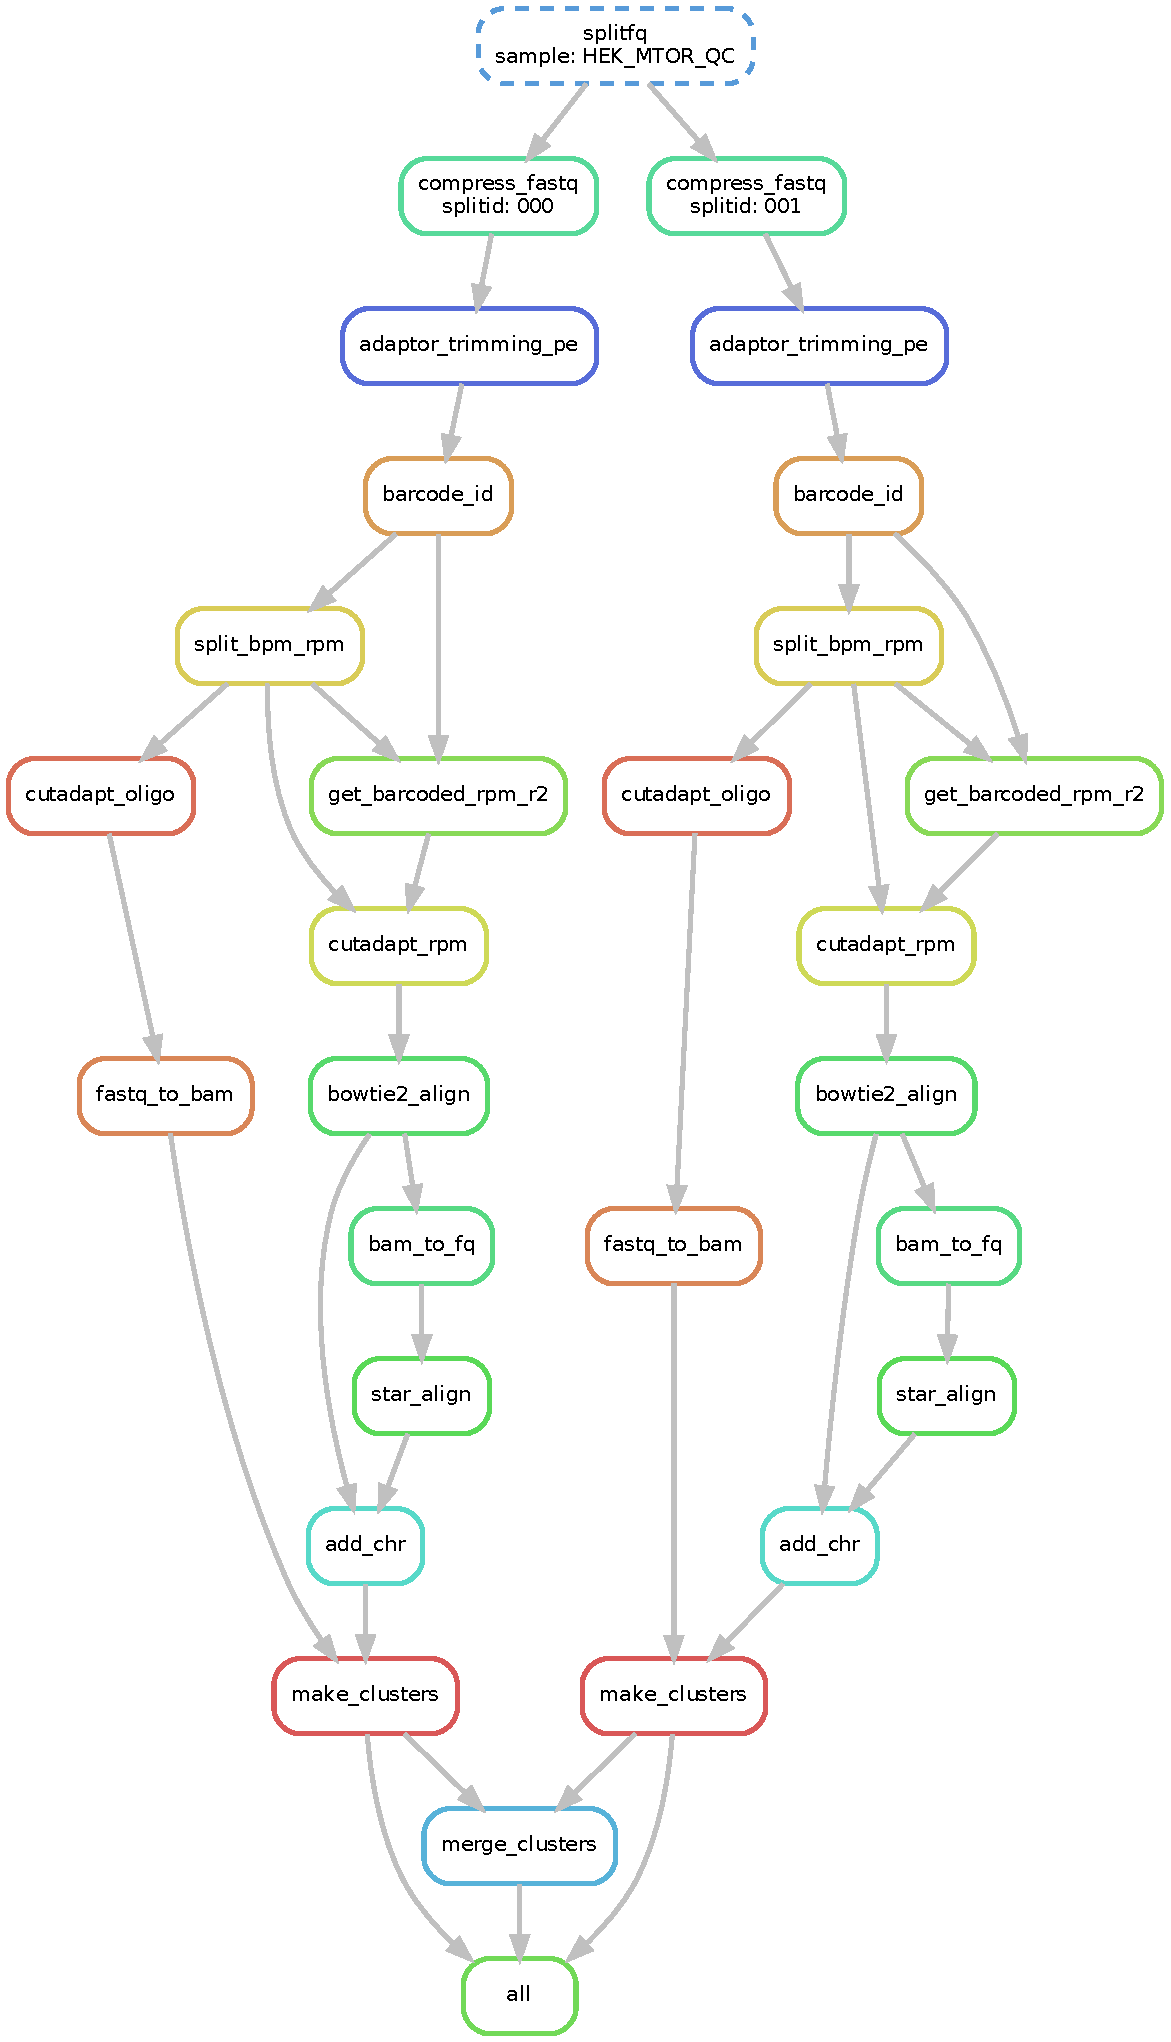
\includegraphics[scale=0.5]{../pipeline/dag.pdf}
        \caption[short]{Example of directed acyclic graph (DAG) for preprocessing pipeline with \texttt{num\_chunks}$=2$}
    \end{figure}

    \noindent Each color corresponds to a different rule. To see the contents of each rule you can view the \texttt{Snakefile}. The arrows represent the flow of data and the dependencies between rules. A rule will not run until all of its dependencies have successfully completed.

    \subsection{Running the Pipeline}

    \begin{enumerate}
        \item Clone the repository from GitHub onto the cluster. (\texttt{git clone https://github.com/mjlab-Columbia/spidr.git})
        \item Change directories into the pipeline directory (\texttt{cd pipeline}).
        \item Modify the \texttt{cluster.yaml} file to reflect your account ID, email, and other parameters. The email written in the \texttt{cluster.yaml} will be the one which error emails are sent to. The account ID should be the one that you use to submit jobs to the cluster (\texttt{mjlab} for anyone in the lab).
        \item Modify the \texttt{config.yaml} to specify the locations of the indices you want to use for alignment (bowtie2 and STAR). Set any other parameters as you would like.
        \item Install mamba outside of your home directory and change your 
        \texttt{\$HOME/.bashrc} file to include the path to mamba. This will allow you to use mamba to install the necessary conda packages. This is necessary because Snakemake uses the mamba dependency resolver by default and your home directory is somewhat limited in space and permissions. For more detailed steps see the steps below, otherwise continue.
            \begin{itemize}
                \item Download mambaforge: \\
                curl -L -O "https://github.com/conda-forge/miniforge/releases/latest/download/Mambaforge-$(uname)-$(uname -m).sh"
    
                \item Run the installation script from the same place you downloaded it: \\
                bash Mambaforge-$(uname)-$(uname -m).sh
                \item Follow the prompts on screen and when asked where to install mamba, specify a location outside of your home directory. I chose \texttt{/burg/mjlab/users/dsg2157/cli-tools}.
                \item Edit your \texttt{\$HOME/.bashrc} file to include the following line: \\
                \texttt{export PATH=/burg/mjlab/users/cli-tools/mamba/bin:\$PATH}
            \end{itemize}
        \item Install \texttt{snakemake} in your base environment via \texttt{mamba install -c conda-forge snakemake}. This will allow you to run the pipeline.
        \item Create a folder called \texttt{fastq\_files} and place gzipped fastq files in there.
        \item Run \texttt{python fastq2json.py -f fastq\_files} from the \texttt{pipeline} directory. This will create a \texttt{samples.json} file which will be used by the pipeline to determine which fastq files to run.
        \item For testing purposes, change \texttt{num\_chunks} to 2 in order to test the pipeline more quickly. 
        \item Finally run \texttt{bash run\_pipeline.sh} from the \texttt{pipeline} directory. This will submit the pipeline to the cluster. 
        \item You can check the status of your jobs with \texttt{squeue -u <your\_username>}. You can also generate your own DAG of the pipeline by running \texttt{bash dag.sh}.
    \end{enumerate}

    \section{Postprocessing Pipeline}
    I'm not sure how the post-processing pipeline works to be completely honest, so I'm not comfortable writing documentation for it.

    \section{Downstream Analysis (Ahmed)}
    Not sure where Ahmed's code and figures are located.

    \section{Downstream Analysis (Darvesh)}
    Below is a comparison of the ENCODE data to the outputs of SPIDR. Specifically, we compare the transcript proportion as given by the supplementary data of ENCODE along with the ENCODE raw data processed through the same pipeline as the SPIDR data.
    \begin{figure}[!ht]
        \centering
        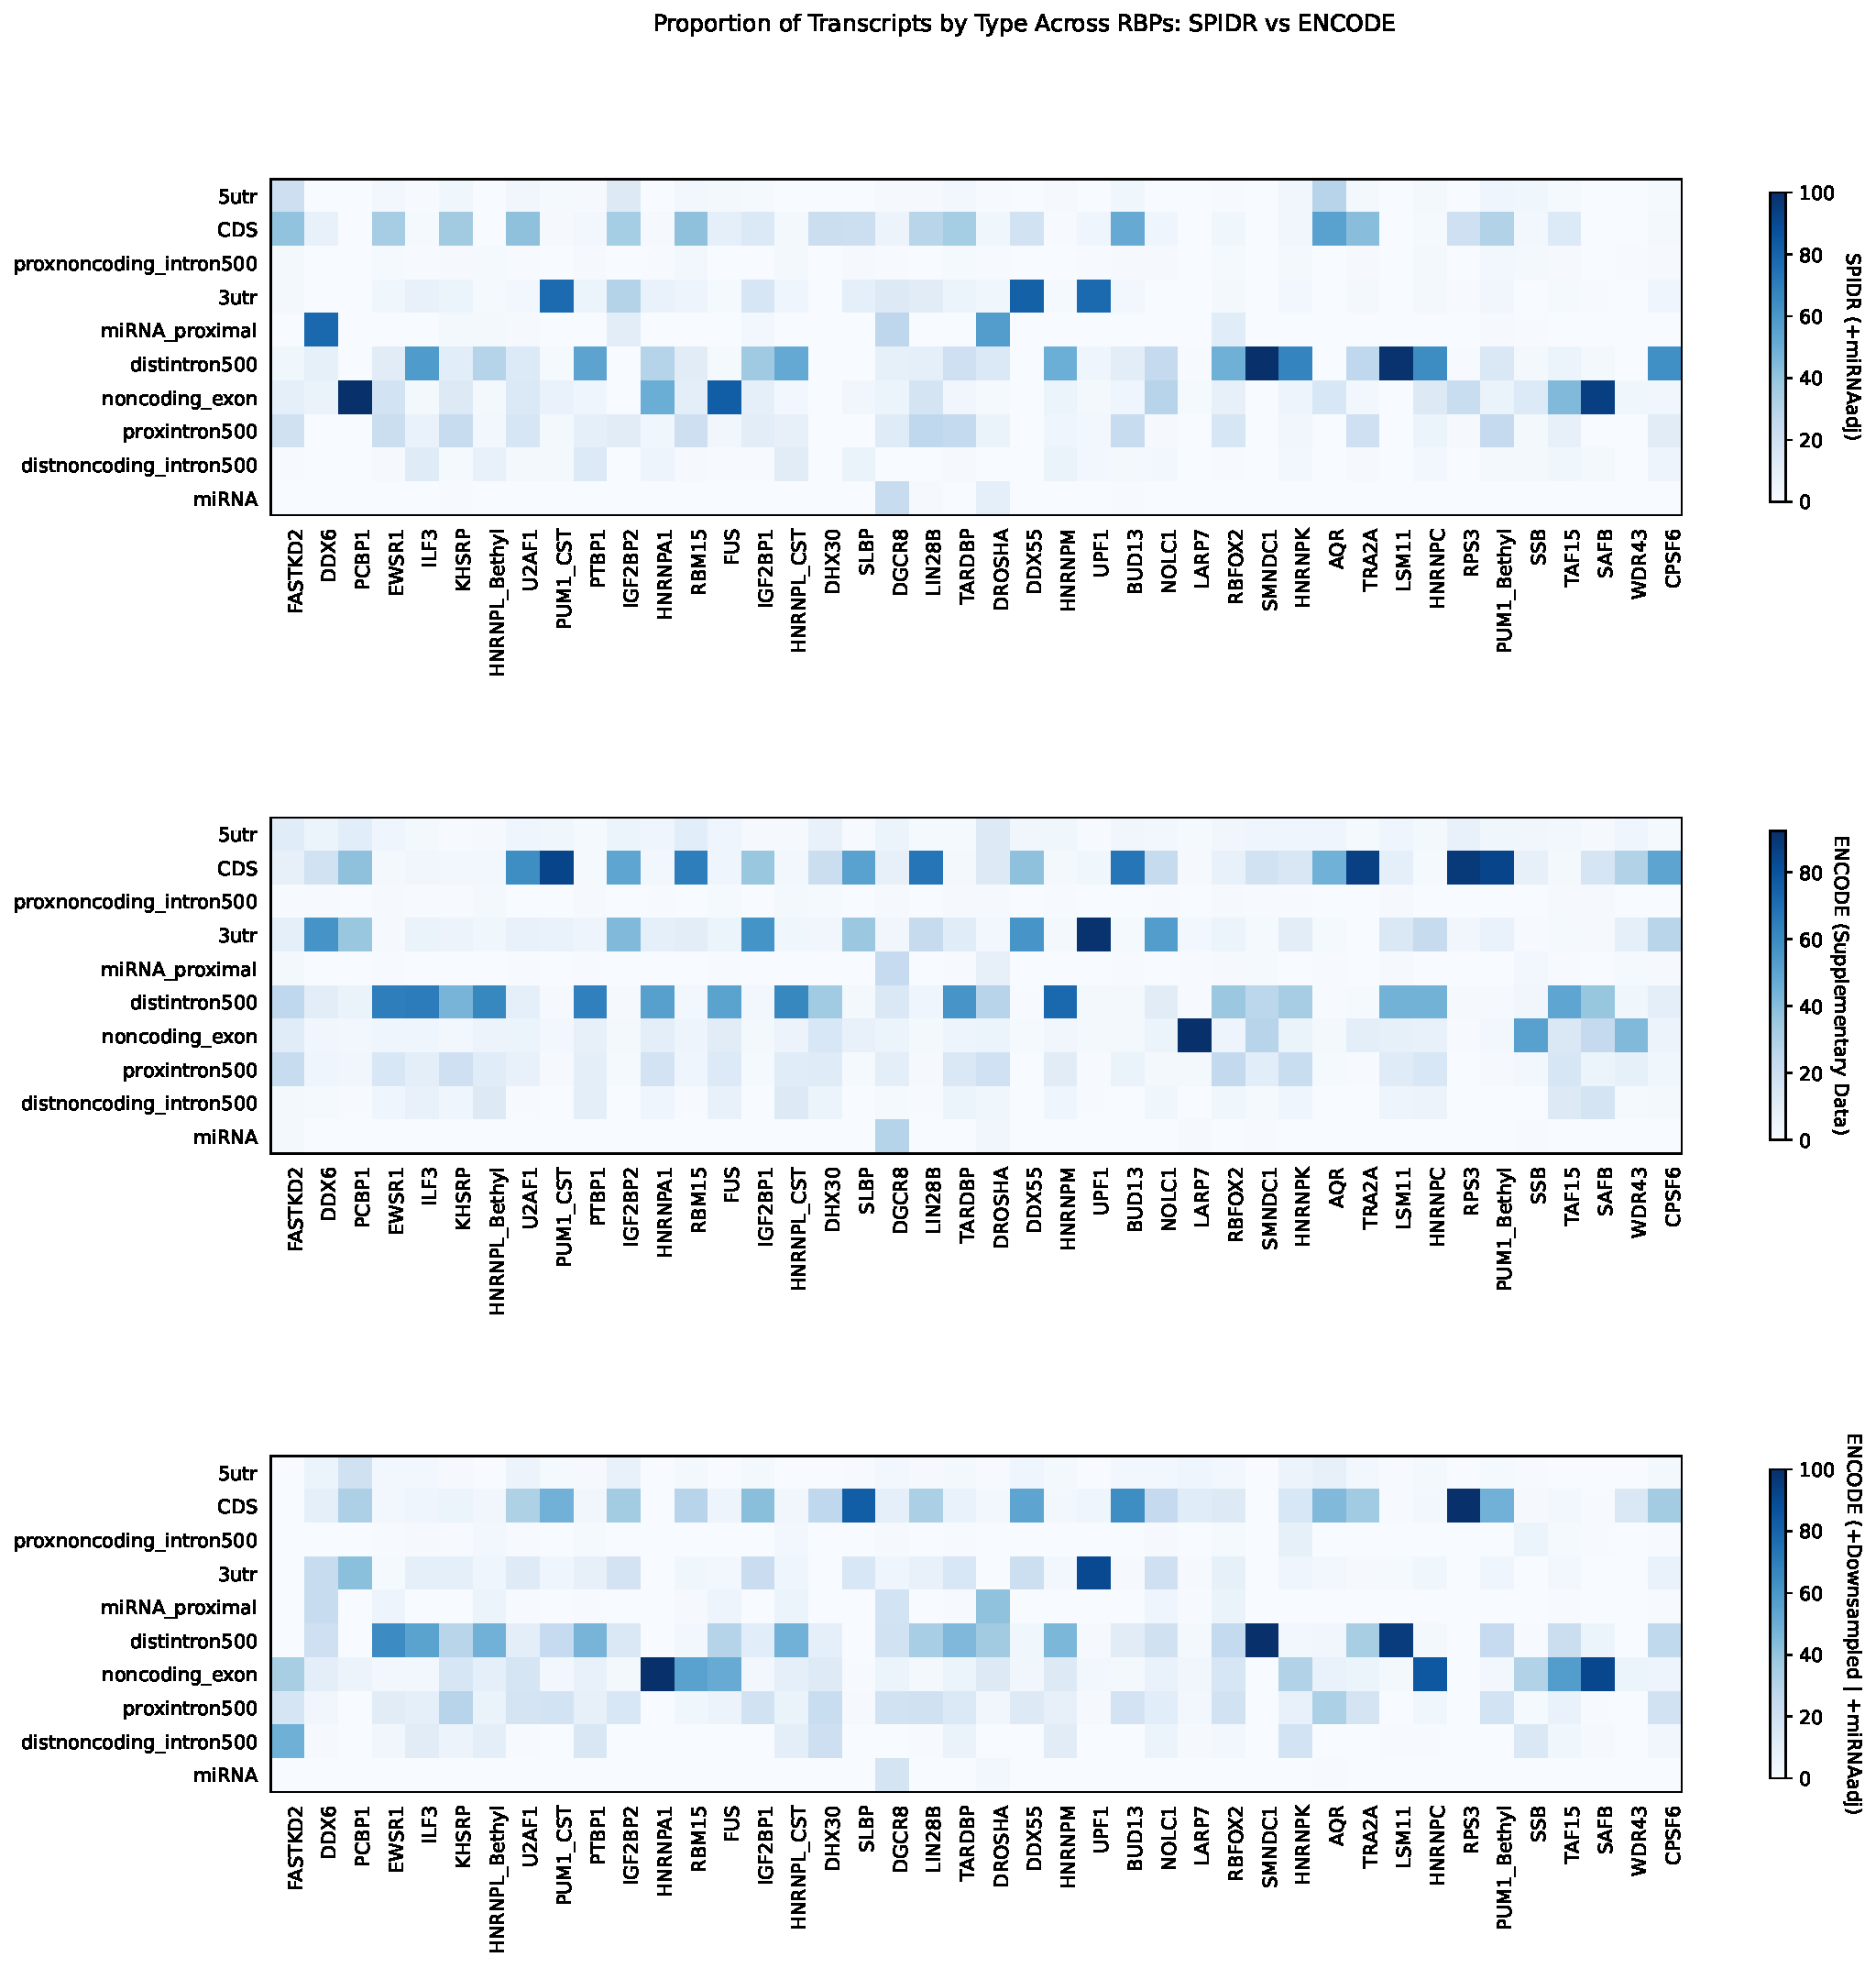
\includegraphics[scale=0.4]{../figures/heatmap_spidr_vs_encode_miRNAadj.pdf}
        \caption[short]{Comparing ENCODE to SPIDR }
    \end{figure}
    
    \noindent We also compared the distribution of imputed transcript proportions versus the true transcript proportions. Essentially, we wanted to ensure that our observed transcript proportions were significantly different from those that we would expect by chance. Indeed, this was the case.
    \begin{figure}[!ht]
        \centering
        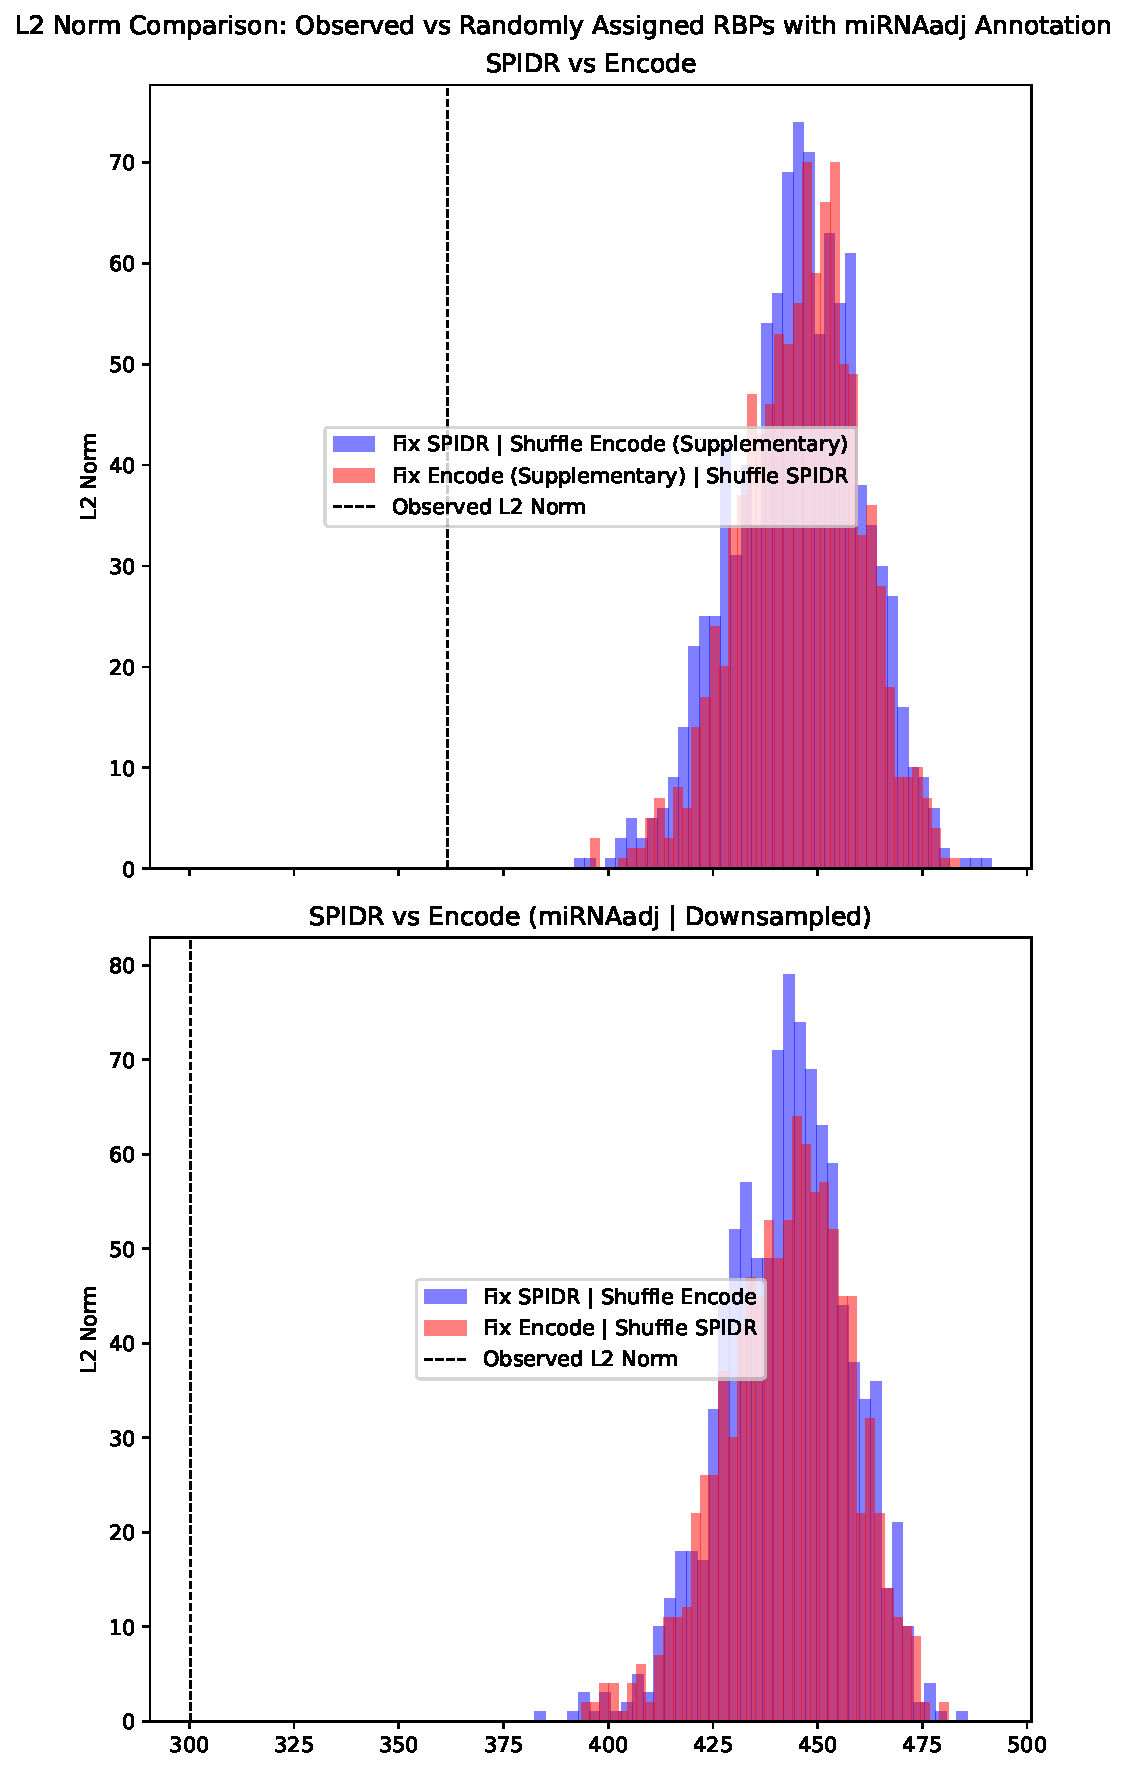
\includegraphics[scale=0.6]{../figures/l2-shuffle-impute-with-miRNAadj.pdf}
        \caption[short]{Comparing ENCODE to SPIDR }
    \end{figure}
\end{document}